\documentclass[11pt,border=5pt]{standalone}
\usepackage{fontspec}
\setmainfont{cmunrm.otf}[BoldFont=cmunbx.otf,ItalicFont=cmunti.otf,BoldItalicFont=cmunbi.otf]
\usepackage{amsmath}
\usepackage{unicode-math}
\setmathfont{NewCMMath-Regular.otf}
\usepackage{tikz}
\usetikzlibrary{arrows.meta,patterns,angles,quotes}
\begin{document}
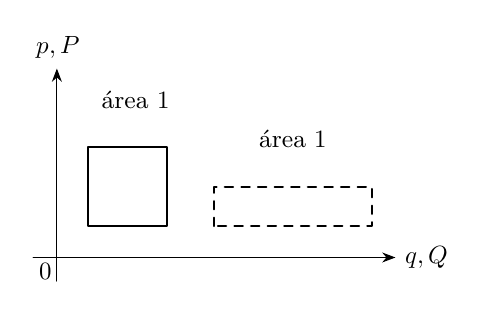
\begin{tikzpicture}[>=Stealth,font=\small,line cap=round,line join=round]
\draw[->,thin] (-0.3,0) -- (4.3,0) node[pos=1,right] {$q,Q$};
\draw[->,thin] (0,-0.3) -- (0,2.4) node[pos=1,above] {$p,P$};
\node at (-0.14,-0.18) {$0$};
\draw[thick] (.4,.4) rectangle (1.4,1.4);\draw[thick,dashed] (2,.4) rectangle (4,.9);
\node at (1,2) {área $1$};
\node at (3,1.5) {área $1$};

\end{tikzpicture}
\end{document}
